\documentclass{article}
\usepackage{xr}
\usepackage{ijcai26}

\usepackage{times}
\usepackage{soul}
\usepackage{url}
\usepackage[hidelinks]{hyperref}
\usepackage[utf8]{inputenc}
\usepackage[small]{caption}
\usepackage{graphicx}
\usepackage{amsmath}
\usepackage{booktabs}
\usepackage{multirow}
\usepackage{xcolor} % 可以保留，即使当前没用到
\usepackage{amsfonts}

\urlstyle{same}

\pdfinfo{
/TemplateVersion (IJCAI.2026.0)
/Title (Cardio-Hybrid Net: Uncertainty-Aware LLM-Guided Multimodal Prediction of Cardiovascular Deterioration in Critical Care)
/Author (Paper ID 218)
/Subject (Artificial Intelligence; Paper ID 218)
}

\title{Cardio-Hybrid Net: Uncertainty-Aware LLM-Guided Multimodal\\
Prediction of Cardiovascular Deterioration in Critical Care}

% Multiple author syntax (remove the single-author syntax above and the \iffalse ... \fi here)
\iffalse
\author{
Yi Zheng$^1$
\and
Fei Zhao$^1$\and
Chi Dong$^1$\And
Xiaohua Liu$^{1,2}$\And
Ming Yang$^3$\And
Chengkai Zhang$^2$\And
Xiangfeng Luo$^2$\\
\affiliations
$^1$School of Artificial Intelligence, Jianghan University, Wuhan, Hubei, 430056, China.\\
$^2$State Key Laboratory of Precision Blasting, Jianghan University, Wuhan, Hubei, 430056, China.\\
$^2$Wuhan Sixth Hospital, Wuhan, Hubei, 430019, China.\\
\emails
yizheng@jhun.edu.cn,\{zhaofei, dongchi\}@stu.jhun.edu.cn,
xiaohualiu@jhun.edu.cn,
zhangchengkai\_efeelture1@gmail.com,
xiangfengluo@qq.com.
}
\fi
\author{
    Paper ID 218
    \affiliations
    Anonymous IJCAI Submission
}

\externaldocument{cardio}
\begin{document}

\title{Supplementary Material}
\maketitle

\appendix

\section{Additional Results and Case Studies}
\label{app:additional_results}

\subsection{Case Reports}

\begin{figure*}[htbp!]
  \centering
  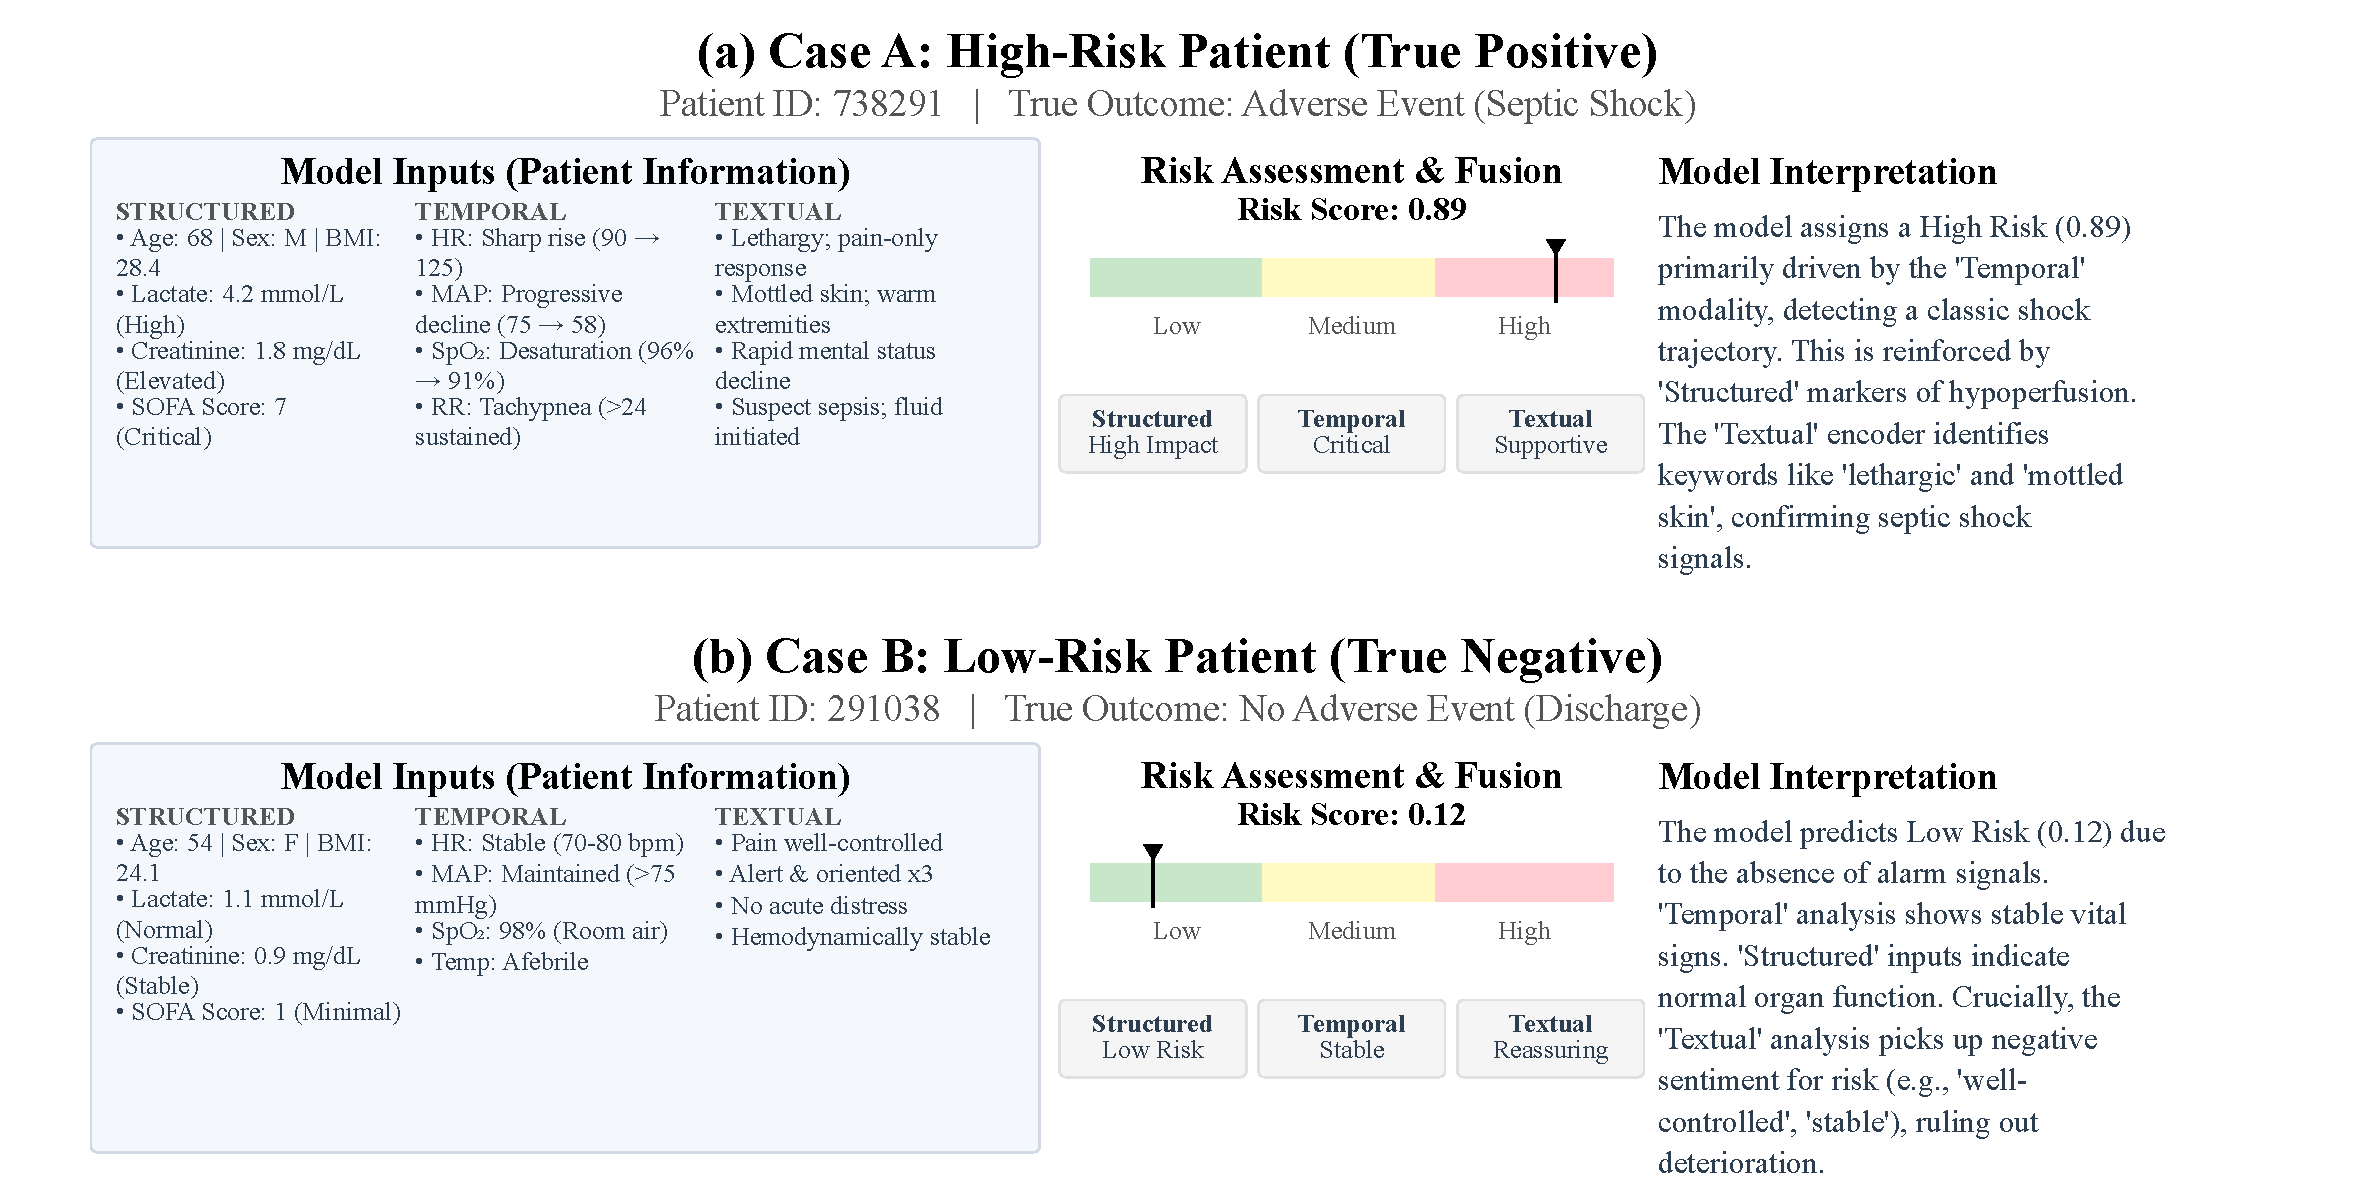
\includegraphics[width=0.95\linewidth]{figs/case-study.pdf}
  \caption{Representative case studies illustrating multimodal trajectories, attention patterns, retrieved similar cases, and LLM-assisted reasoning for a high-risk true positive and a low-risk true negative.}
  \label{fig:case-study}
\end{figure*}

Figure~\ref{fig:case-study} illustrates two cases: a high-risk true positive in whom both the time series and notes strongly indicate deterioration, and a low-risk true negative with stable trends and reassuring narrative.
In the high-risk case, the LLM-backed consultation reinforces the local model's elevated risk estimate and provides a rationale that emphasizes the same multimodal signals as the attention mechanism.
In the low-risk case, the router does not trigger LLM consultation because the local model's prediction is confident and well calibrated.


\subsection{Detailed Architecture of Cardio-Hybrid Net}

\begin{figure*}[htbp!]  
  \centering
  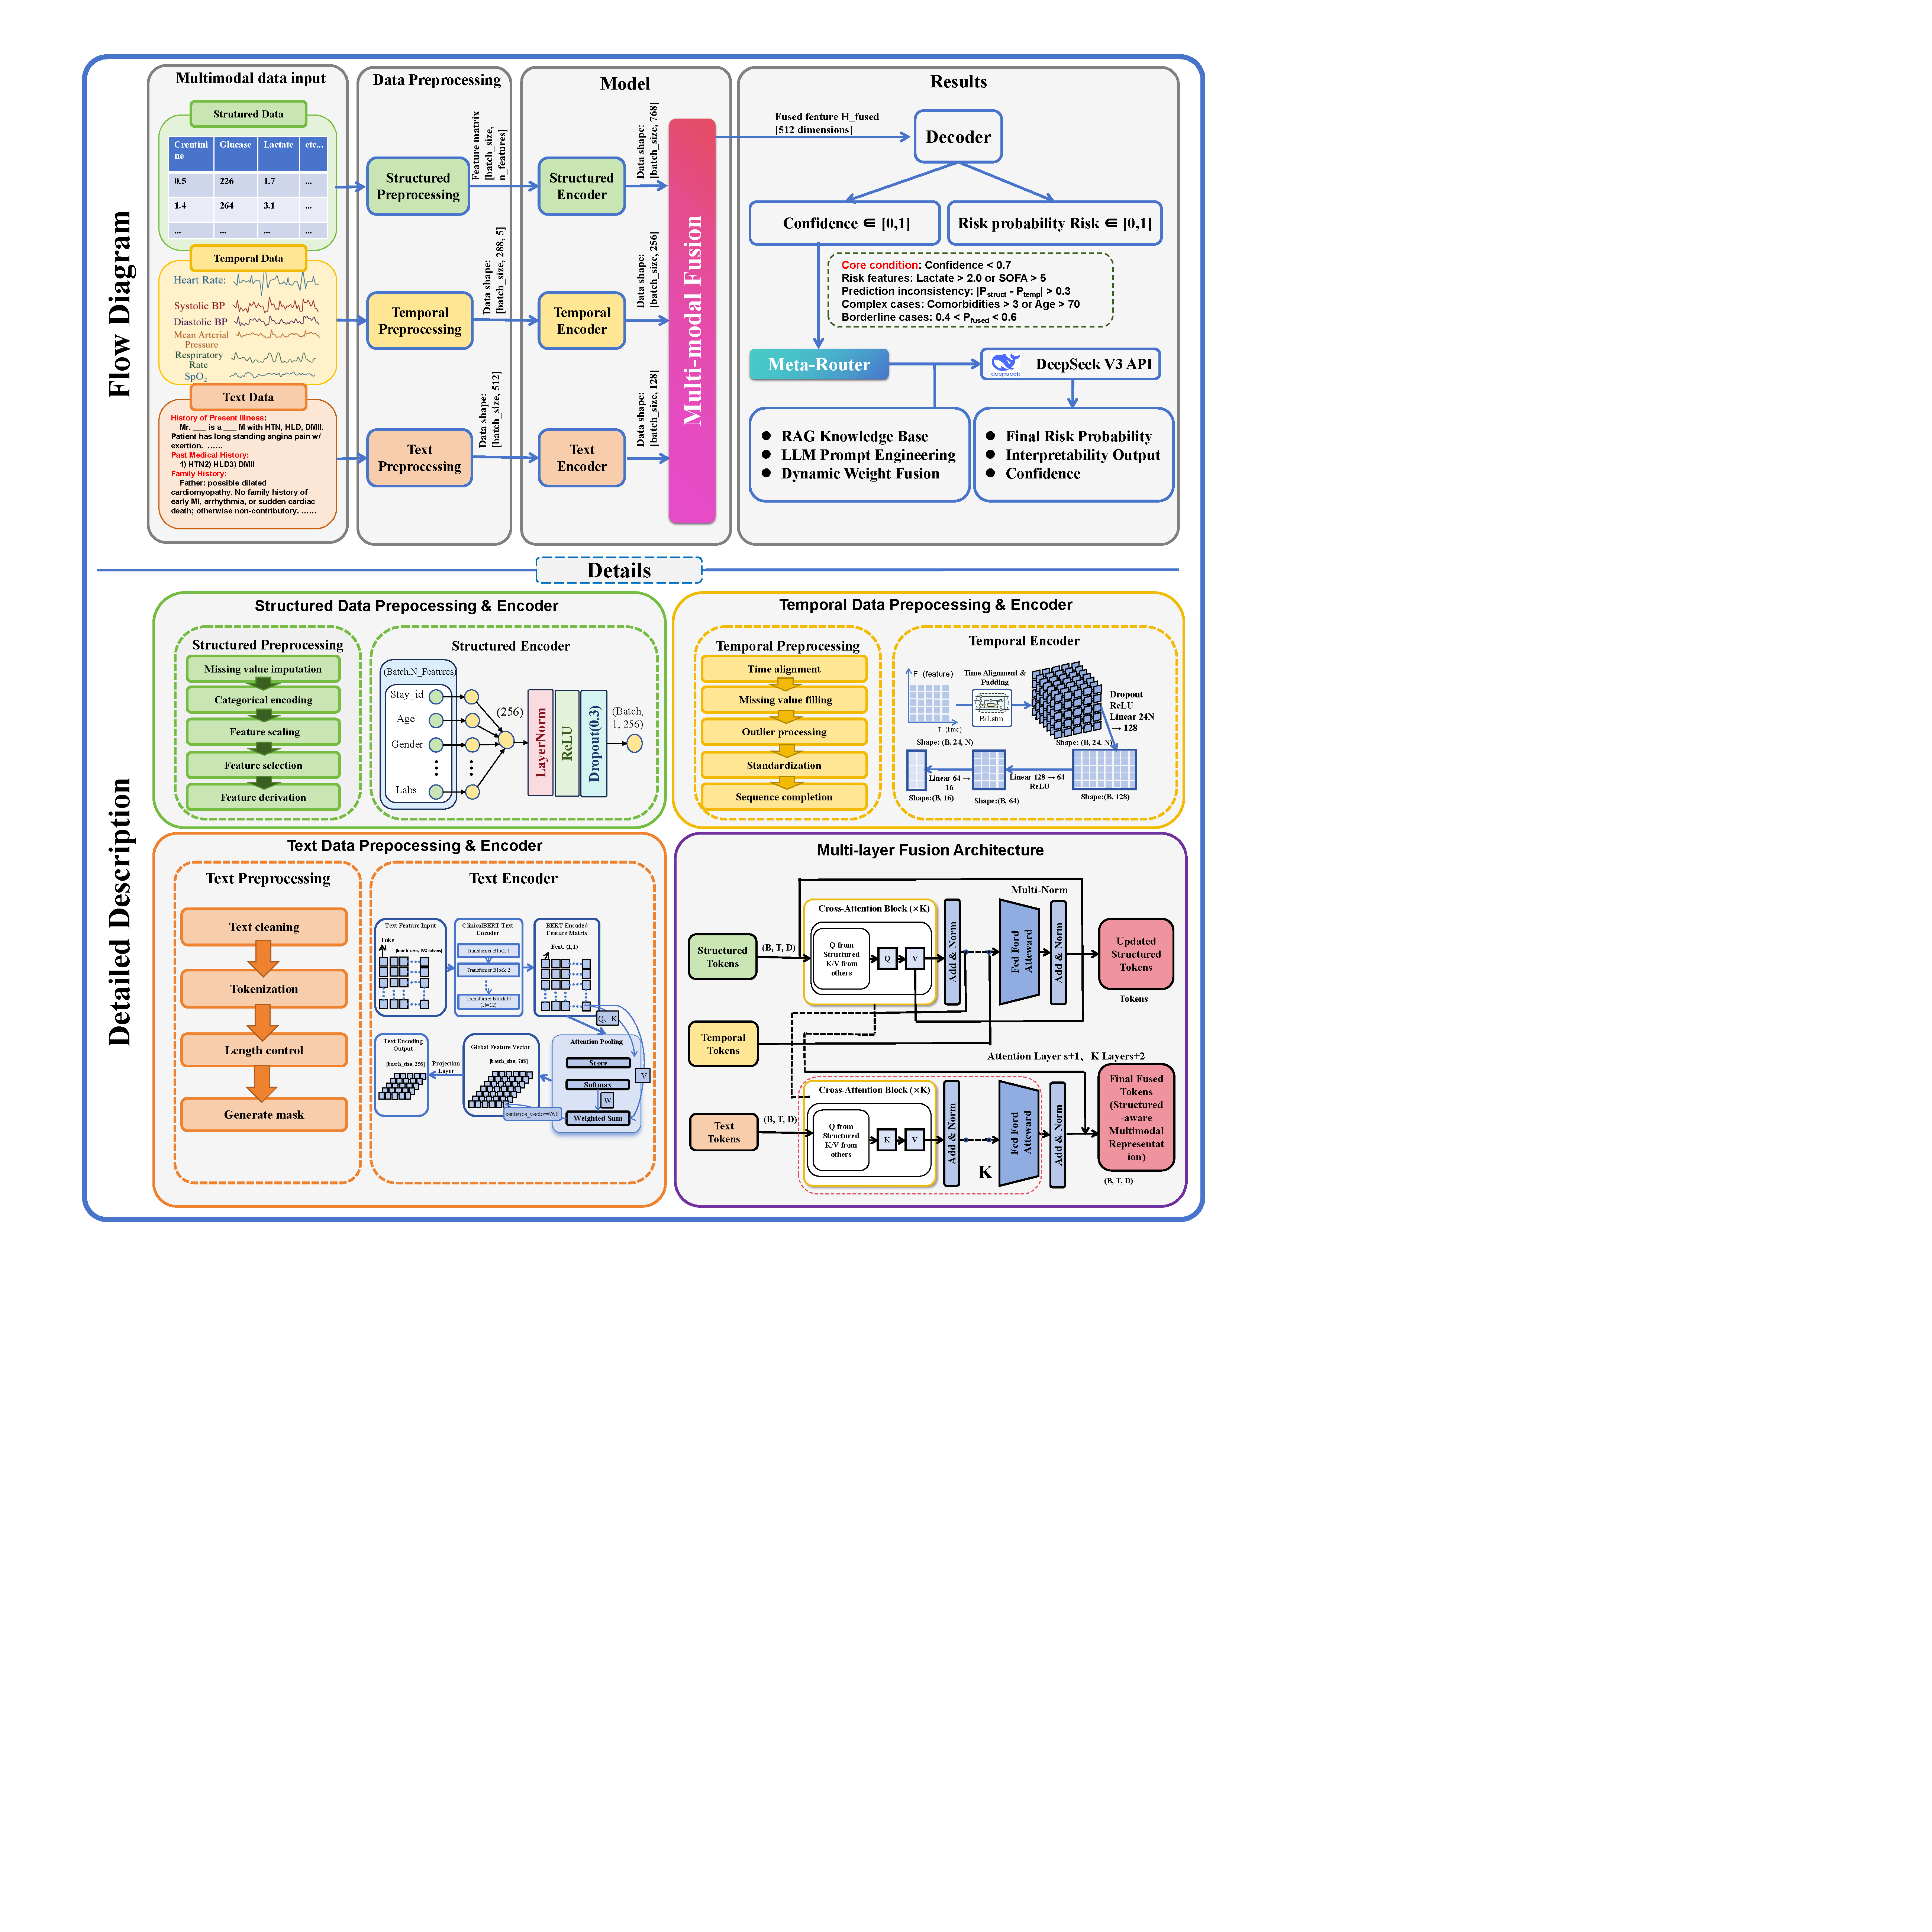
\includegraphics[width=0.9\textwidth]{figs/architecture_detail.pdf}
  \caption{Overall architecture of Cardio-Hybrid Net, including tri-stream encoders, cross-modal attention, uncertainty estimation, and LLM routing.}
  \label{fig:architecture_detail}
\end{figure*}



\bibliographystyle{named}
\bibliography{refs}

\end{document}
